%---------------------------------------------------
% کلاس سند: article برای اسناد متنی، با اندازه کاغذ A4 و فونت پایه 16
\documentclass[a4paper,16pt]{article}

% بسته‌های ریاضی برای معادلات و نمادهای پیشرفته
\usepackage{amsmath, amssymb, amstext}

% بسته رنگ برای استفاده از رنگ در متن یا محیط‌ها
\usepackage{xcolor}

% بسته گرافیک برای درج تصاویر
\usepackage{graphicx}

% تنظیمات حاشیه صفحه
\usepackage{geometry}

% بسته لینک‌دهی (هایپرلینک‌ها)
\usepackage{hyperref}

% بسته صفحه‌آرایی برای تنظیم هدر و فوتر
\usepackage{fancyhdr}


% بسته xepersian برای پشتیبانی از زبان فارسی با XeLaTeX


% تعیین فونت فارسی (فایل فونت باید موجود باشد یا در سیستم نصب باشد)
\usepackage{xepersian}
\settextfont{B Nazanin}

\setlatintextfont{Times New Roman}

% تنظیم اندازه حاشیه‌ها از هر طرف برابر با 1 اینچ
\geometry{margin=1in}

% تنظیم سبک fancy برای سربرگ و پاورقی
\pagestyle{fancy}

% سمت چپ هدر: مشخص‌کننده سری تمرین و نام درس
\lhead{تمرین سری پنجم درس مکانیک تحلیل }

% وسط هدر: نام دانشکده
\chead{دانشکده فیزیک دانشگاه صنعتی خواجه نصیرالدین طوسی}

% سمت راست هدر: تاریخ روز به‌صورت خودکار
\rhead{\today}

% پایین صفحه: شماره صفحه
\cfoot{\thepage}

% شروع سند
\begin{document}
	
	% صفحه عنوان (بدون هدر و فوتر)
	\thispagestyle{empty}
	\begin{center}
		% لوگوی دانشگاه (باید فایل تصویر در مسیر پروژه باشد)
		
\includegraphics[width=0.5\textwidth]{../../../images/image-E_5/image-1.png} \\[10pt] 
		
		% عنوان سند
		\textbf{\LARGE عنوان:تمرین سری پنجم}\\[20pt]
		
		% نیم‌سال تحصیلی
		\textbf{\LARGE نیم‌سال تحصیلی:4041 }\\[10pt]
		
		% نام مدرس درس
		\textbf{\Large مدرس: دکتر محمد انصاری‌فرد}\\[10pt]
		
		% مبحث تمرین 
		\textbf{\Large مبحث تمرین:حساب تغییرات   }\\[10pt]
		
		% مهلت تحویل تمرین
		\textbf{\Large مهلت تحویل:۹دی }
	\end{center}
	
	% صفحه جدید برای ادامه سند
	\newpage
	
	% ایجاد فهرست مطالب به‌صورت خودکار (براساس \section و \subsection و ...)
	\tableofcontents
	\newpage
	
	
	\section{سوال اول}
	
	ثابت کنید کوتاه‌ترین مسیر بین دو نقطه ثابت  
	\[
	A(x_1,y_1), \qquad B(x_2,y_2)
	\]
	در صفحه اقلیدسی، یک خط راست است.
	
	\section{سوال دوم}
	
	سطحی دوار را در نظر بگیرید که از دوران منحنی \( y(x) \) حول محور \( x \)
	ایجاد می‌شود.  
	این منحنی از دو نقطه انتهایی ثابت
	\[
	(x_1, y_1), \qquad (x_2, y_2)
	\]
	می‌گذرد.
مسئله وردشی را به‌گونه‌ای فرموله کنید که تابع \( y(x) \) به‌عنوان تابع
	اختیار انتخاب شود و مساحت سطح دوار کمینه گردد.
	
	\section{سوال سوم}
	
	پرتوی نور را در نظر بگیرید که از محیطی با ضریب شکست \( n_1 \)
	وارد محیط دیگری با ضریب شکست \( n_2 \) می‌شود.
	فرض کنید مرز بین دو محیط یک صفحه صاف است و پرتو نور از نقطه ثابت\lr{A}
	در محیط اول به نقطه ثابت\lr{B}
	در محیط دوم می‌رسد.با بهره‌گیری از اصل فرما، یعنی کمینه بودن زمان حرکت نور،
	تابعی برای زمان پیمایش نور تعریف کرده و با کمینه‌سازی آن
	قانون شکست نور (قانون اسنل) را استخراج کنید.
	\begin{figure}[h]
		\centering
		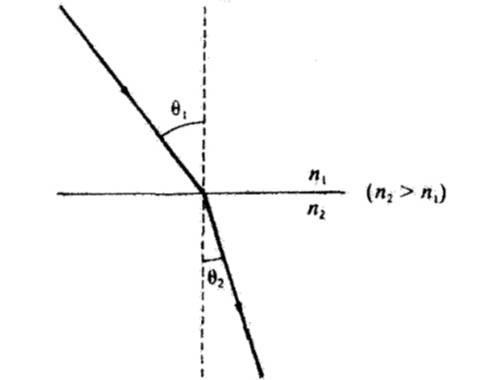
\includegraphics[width=0.5\textwidth]{../../../images/image-E_5/image-2.jpg}
	\end{figure}
	
	\section{سوال چهارم}
	 
	یک استوانه) با شعاع \( R \) و ارتفاع \( H \) را در نظر بگیرید
	که حجم آن مقدار ثابتی برابر \( V \) است.نسبت
	\[
	\frac{R}{H}
	\]
	را به‌دست آورید به‌گونه‌ای که مساحت کل سطح استوانه کمینه شود.
	
	\section{سوال پنجم}
	یک کابل انعطاف‌پذیر و سبک بین دو نقطه ثابت 
	\[
	A(0,0) \quad \text{و} \quad B(L,H)
	\] 
	در صفحه قائم آویزان شده است.  
	نیروی گرانش یکنواخت \( g \) اثر می‌کند و کابل فقط **وزن خود** را دارد.\\مسئله: مسیر کابل را بیابید به‌گونه‌ای که **انرژی پتانسلی گرانشی کل** کمینه شود.
	
	
	\vspace{10pt}
	\textbf{موفق باشید.}
\end{document}
